\section*{Abstract}
The study of stellar clusters within the Galaxy serves an important role in understanding the Galaxy’s physical and chemical characteristics. Open stellar clusters are defined as gravitationally-bound groups of stars born from a single, homogeneous molecular cloud, typically composed of a single stellar population. This allows us to measure physical parameters such as a cluster’s age, metallicity, distance, and extinction, which can be determined through photometric data of resolved cluster members. Studies of Galactic clusters have seen a significant boon in recent years with the advent of Gaia, whose unmatched astrometric precision has allowed for the identification of thousands of new stellar clusters, as well as refining membership lists for previously identified clusters.

This doctoral thesis project makes use of Gaia DR3 (and DR4 in the near future) data to update and expand the membership lists from the Hunt \& Reffert (2024) and the Unified Cluster Catalog (UCC). By using HDBSCAN we identify an additional population of faint stars for each cluster, extending beyond the main clusters’ cores. We determine each cluster’s physical parameters using both isochrone fitting methods such as ASteCA, as well as a neural network trained on observational Hertzsprung-Russell diagrams in various passbands (Gaia, 2MASS, WISE, SDSS), including Johnson-Cousins UBVRI passbands from observations made at the Observatorio Astronómico Universitario – San Pedro Martir. Multi-band observations, as well as the recovery of previously unreported faint (G > 18) members, will help us break degeneracies present in the parameter space responsible for parameter discrepancies across catalogs.

\section{Introduction}
Given that stars make up the fundamental blocks of the Galaxy, stellar clusters (SCs) therefore act as important astrophysical laboratories ideal for understanding It's dynamics and structure. Stars are well known to be born in cohorts within molecular clouds, dissolving into the interstellar medium to form the field stars that can be seen today. From current star formation theory we know that the youngest of these clusters where formed from a singular burst of star formation, and are therefore referred to as \textit{simple stellar populations} (SSPs), groups of chemically homogeneous stars \autocite{huangDrivingFactorsMultiple2024}. These groups are known as \textit{open clusters} (OCs) due to their loosely-bound and irregular appearance. OCs also tend to exhibit lower total stellar masses, and are primarily located in the Galactic disk \autocite{zwartYoungMassiveStar2010a}. OCs can be used as tracers for studying the Galactic spiral structure \autocite{dias58OpenClusters2022}.

Globular clusters (GCs), on the other hand, are high-density collections of stars, distributed throughout the Galactic halo. GCs are found to be in a more stable virial state, with an older age distribution as well as higher dynamical timescales, which contributes to their spherically symmetrical appearance. As a result of their larger age, GC populations tend to be more complex, to the point that they sometimes cannot be properly described as a SSP; chemical abundance variations between stars in a single GC indicates \textit{multiple stellar populations} (MPs) with later-generation stars showing distinct chemical compositions \autocite{huangDrivingFactorsMultiple2024}. Although they have historically been studied as a separate category from OCs, current models do not discriminate between either OCs or GCs for describing their dynamics and compositions \autocite{krumholzStarClustersCosmic2019}.

% CMD analysis
Photometric studies of SCs involve fitting synthetic isochrones to color--magnitude diagrams (CMDs). Each isochrone depends on the given age, metallicity, distance, and reddening parameters; each parameter is simultaneously adjusted such that the dispersion around the resulting isochrone is minimized. Stellar isochrones are generated with codes such as PARSEC \autocite{bressanPARSECStellarTracks2012} for a given grid of parameters, which are then fit through visual analysis of the CMDs (which inevitably introduces a level of bias into the solution) or by automated methods such as ASteCA \autocite{perrenASteCAAutomatedStellar2015} or a cross-entropy optimization algorithm with a likelihood function defined by the distance of each point to the nearest point on the isochrone \autocite{monteiroFittingIsochronesOpen2010}. Recent efforts have been made in the characterization of open clusters in today's age of Big Data, with machine learning tools being made to characterize each cluster from the observed CMDs \autocite{huntImprovingOpenCluster2023a,cavalloParameterEstimationOpen2023}. Large samples of Galactic SCs enable the morphological and chemical distribution through the Galaxy \autocite{gaiacollaborationGaiaDataRelease2023b,huMetallicitiesOldOpen2025}.

% memberships
In order to properly characterize a SC, it's member stars must be properly identified to avoid including field stars not bound to the cluster in question for the ensuing CMD analysis. As a result, cluster membership determination algorithms have received a large amount of attention in recent years. Algorithms like DBSCAN and the related HDBSCAN have been used in recent studies for identifying of cluster members \autocite{huntImprovingOpenCluster2021,longInvestigating16Open2023}. 

\section{Objectives}
Although a variety of studies have been done using CMDs from other catalogs, few studies include observations in near-ultraviolet filters due to the demanding photometric conditions (as a result of atmospheric sensitivity) required to obtain reliable measurements for a cluster's metallicity and age. For this project, we will exploit over 20 years of UBVRI observations of over 1700 resolved Galactic clusters (both GCs and OCs), which can be used to provide reliable measurements of the clusters' fundamental parameters with stronger model constraints than is otherwise possible without UBV observations \autocite{kavirajBetterAgeEstimation2007}. The observations from the \textit{Observatorio Astron\'omico Nacional -- San Pedro M\'artir} (hereafter referred to as SPM) are complemented with photometry obtained from all-sky surveys when available, crossmatching the Gaia observations with GALEX, 2MASS, PAN-STARRS, SDSS, and WISE.

% Although this has been a troublesome task in the past, the advent of Gaia\textemdash with the third data release (DR3) being the latest offering \autocite{gaiacollaborationGaiaDataRelease2023a}\textemdash has greatly improved membership determination through highly accurate astrometric parameters. 

The project's key objectives are outlined as follows:

\begin{itemize}
    \item Determine stellar cluster memberships using high quality astrometric data.
    \item Develop new tools for the efficient and accurate characterization of cluster CMDs.
    \item Use newly developed tools for determining stellar and cluster parameters of SCs and SC candidates using observations from SPM, supplemented with observations from external catalogs: 2MASS, WISE, GALEX, Gaia, PAN-STARRS, and SDSS when available.
\end{itemize}

\section{Observations Sample}
As previously mentioned, we have cataloged over 1700 clusters observed over the course of 3212 individual observations dating back to the year 2001. Each observational campaign focuses either on the suspected cluster members, or the foreground or background stars. Doing a preliminary cross-match with the \textit{Unified Cluster Catalog} (UCC; \cite{perrenUnifiedClusterCatalogue2023}) shows over 300 clusters not identified in the UCC, with some having been identified as asterisms (physically unrelated groups of observed stars). As part of the initial data exploration step of the methodology, a more in-depth review of the published literature will be needed to determine the characterization already performed for each cluster in the sample. 

As can be seen in Figure \ref{fig:mw-distribution}, our observations encompass a dense sample the Solar neighborhood, both spatially as well as characterization quality from the UCC UTI metric, providing a good opportunity to improve the worst-scoring clusters and provide a uniform study of the stellar parameter spatial distributions. Thanks to the photometric conditions of at SPM, stars up to a magnitude of $\sim  21$ can be recorded, allowing for a deeper high quality measurement of SC members. This will allow us to obtain quality photometric measurements for a higher amount of low luminosity members, thus reducing selection bias effects as a result of incomplete sampling of low mass members.

\begin{figure}[!ht]
    \centering
    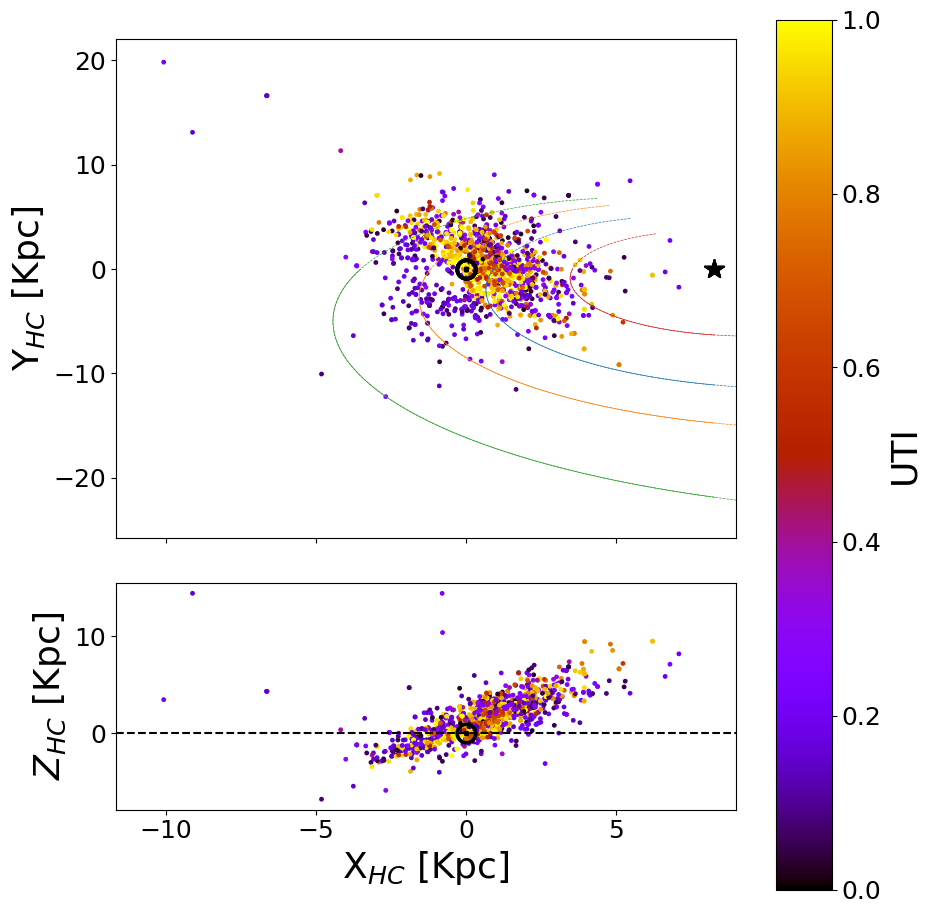
\includegraphics[width=0.85\linewidth]{figures/SPM Milky Way Clusters.png}
    \caption{Spatial distribution of observed SCs in the Galaxy in the Solar neighborhood.}
    \label{fig:mw-distribution}
\end{figure}

\section{Methodology}

\subsection{Cluster Membership}
Proper characterization of a stellar cluster is highly dependent on accurate discrimination of field stars from cluster members. Using Gaia DR3 (GDR3) astrometric data \autocite{gaiacollaborationGaiaDataRelease2023a} as input into clustering algorithms like FFC we will determine stellar cluster memberships with a high degree of confidence. In order to improve efficiency, we will be performing a focused search; for the SCs that have a published solution we will be using a multiple of the core radius to extract an appropriate number of sources from GDR3. For the clusters with no reliable measurement of the core radius, a similar process of source selection will be applied, albeit with a less informative initial heuristic. 

For this project, we have developed a pipeline around the HDBSCAN clustering algorithm to be used on the Gaia 5D astrometric phase space ($\alpha, \delta, \omega, \mu_{\alpha} \cos{\delta}, \mu_{\delta}$), normalized to avoid the different scales of each parameter to overpower the other four dimensions. No photometric magnitude quality cut was imposed so as to avoid removing an otherwise valid faint cluster member, instead using astrometric quality flags for retaining reliable observed stars. To take advantage of each cluster's published information, we retrieve a field from Gaia DR3 of a few times larger than the tidal radius of each cluster, with the expectation that HDBSCAN can capture members farther away from the cluster's core due to its insensitivity to spherical symmetry. 
% Figure \ref{fig:hdbscan-example} shows the results of applying this pipeline to the field surrounding the OC UBC 409, in which we recover several low-mass faint members previously unreported in the literature.

% \begin{figure}[!ht]
%     \includegraphics[width=\linewidth]{figures/HDBSCAN Example.png}
%     \caption{Example of newly retrieved members using HDBSCAN on the OC UBC 409. The newly proposed members reach farther into the low mass star regime, while maintaining a good overlap with the prevously reported members in the literature.}
%     \label{fig:hdbscan-example}
% \end{figure}